\documentclass[twoside]{book}

% Packages required by doxygen
\usepackage{fixltx2e}
\usepackage{calc}
\usepackage{doxygen}
\usepackage[export]{adjustbox} % also loads graphicx
\usepackage{graphicx}
\usepackage[utf8]{inputenc}
\usepackage{makeidx}
\usepackage{multicol}
\usepackage{multirow}
\PassOptionsToPackage{warn}{textcomp}
\usepackage{textcomp}
\usepackage[nointegrals]{wasysym}
\usepackage[table]{xcolor}

% Font selection
\usepackage[T1]{fontenc}
\usepackage[scaled=.90]{helvet}
\usepackage{courier}
\usepackage{amssymb}
\usepackage{sectsty}
\renewcommand{\familydefault}{\sfdefault}
\allsectionsfont{%
  \fontseries{bc}\selectfont%
  \color{darkgray}%
}
\renewcommand{\DoxyLabelFont}{%
  \fontseries{bc}\selectfont%
  \color{darkgray}%
}
\newcommand{\+}{\discretionary{\mbox{\scriptsize$\hookleftarrow$}}{}{}}

% Page & text layout
\usepackage{geometry}
\geometry{%
  a4paper,%
  top=2.5cm,%
  bottom=2.5cm,%
  left=2.5cm,%
  right=2.5cm%
}
\tolerance=750
\hfuzz=15pt
\hbadness=750
\setlength{\emergencystretch}{15pt}
\setlength{\parindent}{0cm}
\setlength{\parskip}{3ex plus 2ex minus 2ex}
\makeatletter
\renewcommand{\paragraph}{%
  \@startsection{paragraph}{4}{0ex}{-1.0ex}{1.0ex}{%
    \normalfont\normalsize\bfseries\SS@parafont%
  }%
}
\renewcommand{\subparagraph}{%
  \@startsection{subparagraph}{5}{0ex}{-1.0ex}{1.0ex}{%
    \normalfont\normalsize\bfseries\SS@subparafont%
  }%
}
\makeatother

% Headers & footers
\usepackage{fancyhdr}
\pagestyle{fancyplain}
\fancyhead[LE]{\fancyplain{}{\bfseries\thepage}}
\fancyhead[CE]{\fancyplain{}{}}
\fancyhead[RE]{\fancyplain{}{\bfseries\leftmark}}
\fancyhead[LO]{\fancyplain{}{\bfseries\rightmark}}
\fancyhead[CO]{\fancyplain{}{}}
\fancyhead[RO]{\fancyplain{}{\bfseries\thepage}}
\fancyfoot[LE]{\fancyplain{}{}}
\fancyfoot[CE]{\fancyplain{}{}}
\fancyfoot[RE]{\fancyplain{}{\bfseries\scriptsize Generated by Doxygen }}
\fancyfoot[LO]{\fancyplain{}{\bfseries\scriptsize Generated by Doxygen }}
\fancyfoot[CO]{\fancyplain{}{}}
\fancyfoot[RO]{\fancyplain{}{}}
\renewcommand{\footrulewidth}{0.4pt}
\renewcommand{\chaptermark}[1]{%
  \markboth{#1}{}%
}
\renewcommand{\sectionmark}[1]{%
  \markright{\thesection\ #1}%
}

% Indices & bibliography
\usepackage{natbib}
\usepackage[titles]{tocloft}
\setcounter{tocdepth}{3}
\setcounter{secnumdepth}{5}
\makeindex

% Hyperlinks (required, but should be loaded last)
\usepackage{ifpdf}
\ifpdf
  \usepackage[pdftex,pagebackref=true]{hyperref}
\else
  \usepackage[ps2pdf,pagebackref=true]{hyperref}
\fi
\hypersetup{%
  colorlinks=true,%
  linkcolor=blue,%
  citecolor=blue,%
  unicode%
}

% Custom commands
\newcommand{\clearemptydoublepage}{%
  \newpage{\pagestyle{empty}\cleardoublepage}%
}

\usepackage{caption}
\captionsetup{labelsep=space,justification=centering,font={bf},singlelinecheck=off,skip=4pt,position=top}

%===== C O N T E N T S =====

\begin{document}

% Titlepage & ToC
\hypersetup{pageanchor=false,
             bookmarksnumbered=true,
             pdfencoding=unicode
            }
\pagenumbering{alph}
\begin{titlepage}
\vspace*{7cm}
\begin{center}%
{\Large opdracht\+\_\+1\+\_\+3 }\\
\vspace*{1cm}
{\large Generated by Doxygen 1.8.13}\\
\end{center}
\end{titlepage}
\clearemptydoublepage
\pagenumbering{roman}
\tableofcontents
\clearemptydoublepage
\pagenumbering{arabic}
\hypersetup{pageanchor=true}

%--- Begin generated contents ---
\chapter{Class Index}
\section{Class List}
Here are the classes, structs, unions and interfaces with brief descriptions\+:\begin{DoxyCompactList}
\item\contentsline{section}{\hyperlink{classball}{ball} }{\pageref{classball}}{}
\item\contentsline{section}{\hyperlink{classcircle}{circle} }{\pageref{classcircle}}{}
\item\contentsline{section}{\hyperlink{classdrawable}{drawable} }{\pageref{classdrawable}}{}
\item\contentsline{section}{\hyperlink{classline}{line} }{\pageref{classline}}{}
\item\contentsline{section}{\hyperlink{classrectangle}{rectangle} }{\pageref{classrectangle}}{}
\item\contentsline{section}{\hyperlink{classvector}{vector} }{\pageref{classvector}}{}
\item\contentsline{section}{\hyperlink{classwall}{wall} \\*Wall }{\pageref{classwall}}{}
\item\contentsline{section}{\hyperlink{classwindow}{window} }{\pageref{classwindow}}{}
\end{DoxyCompactList}

\chapter{File Index}
\section{File List}
Here is a list of all documented files with brief descriptions\+:\begin{DoxyCompactList}
\item\contentsline{section}{{\bfseries ball.\+hpp} }{\pageref{ball_8hpp}}{}
\item\contentsline{section}{{\bfseries circle.\+hpp} }{\pageref{circle_8hpp}}{}
\item\contentsline{section}{{\bfseries drawable.\+hpp} }{\pageref{drawable_8hpp}}{}
\item\contentsline{section}{{\bfseries line.\+hpp} }{\pageref{line_8hpp}}{}
\item\contentsline{section}{{\bfseries rectangle.\+hpp} }{\pageref{rectangle_8hpp}}{}
\item\contentsline{section}{{\bfseries vector.\+hpp} }{\pageref{vector_8hpp}}{}
\item\contentsline{section}{\hyperlink{wall_8hpp}{wall.\+hpp} }{\pageref{wall_8hpp}}{}
\item\contentsline{section}{{\bfseries window.\+hpp} }{\pageref{window_8hpp}}{}
\end{DoxyCompactList}

\chapter{Class Documentation}
\hypertarget{classcircle}{}\section{circle Class Reference}
\label{classcircle}\index{circle@{circle}}
\subsection*{Public Member Functions}
\begin{DoxyCompactItemize}
\item 
\mbox{\Hypertarget{classcircle_ac6ef4a49c741dcf33e5cf5d05768b450}\label{classcircle_ac6ef4a49c741dcf33e5cf5d05768b450}} 
{\bfseries circle} (\hyperlink{classwindow}{window} \&w, int mid\+\_\+x, int mid\+\_\+y, int radius)
\item 
\mbox{\Hypertarget{classcircle_a0c7d327e326648c249e1ba5439d1a7fa}\label{classcircle_a0c7d327e326648c249e1ba5439d1a7fa}} 
void {\bfseries print} ()
\end{DoxyCompactItemize}


The documentation for this class was generated from the following files\+:\begin{DoxyCompactItemize}
\item 
circle.\+hpp\item 
circle.\+cpp\end{DoxyCompactItemize}

\hypertarget{classfilled__rectangle}{}\section{filled\+\_\+rectangle Class Reference}
\label{classfilled__rectangle}\index{filled\+\_\+rectangle@{filled\+\_\+rectangle}}


\hyperlink{classfilled__rectangle}{filled\+\_\+rectangle}  




{\ttfamily \#include $<$filled\+\_\+rectangle.\+hpp$>$}

\subsection*{Public Member Functions}
\begin{DoxyCompactItemize}
\item 
\hyperlink{classfilled__rectangle_aa8bbee29edffdb5374c6d99ed1bc8073}{filled\+\_\+rectangle} (\hyperlink{classwindow}{window} \&w, int start\+\_\+x, int start\+\_\+y, int end\+\_\+x, int end\+\_\+y)
\begin{DoxyCompactList}\small\item\em The constructor of a \hyperlink{classfilled__rectangle}{filled\+\_\+rectangle}. \end{DoxyCompactList}\item 
void \hyperlink{classfilled__rectangle_aef5f2d6c5d83663512e78a581b400214}{print} ()
\begin{DoxyCompactList}\small\item\em a print function of a \hyperlink{classfilled__rectangle}{filled\+\_\+rectangle} \end{DoxyCompactList}\end{DoxyCompactItemize}


\subsection{Detailed Description}
\hyperlink{classfilled__rectangle}{filled\+\_\+rectangle} 

this library contains a c++ and a h++ file, it contains a constructor and a print function for a \hyperlink{classfilled__rectangle}{filled\+\_\+rectangle} made out of 4 coordinates and a window 

\subsection{Constructor \& Destructor Documentation}
\mbox{\Hypertarget{classfilled__rectangle_aa8bbee29edffdb5374c6d99ed1bc8073}\label{classfilled__rectangle_aa8bbee29edffdb5374c6d99ed1bc8073}} 
\index{filled\+\_\+rectangle@{filled\+\_\+rectangle}!filled\+\_\+rectangle@{filled\+\_\+rectangle}}
\index{filled\+\_\+rectangle@{filled\+\_\+rectangle}!filled\+\_\+rectangle@{filled\+\_\+rectangle}}
\subsubsection{\texorpdfstring{filled\+\_\+rectangle()}{filled\_rectangle()}}
{\footnotesize\ttfamily filled\+\_\+rectangle\+::filled\+\_\+rectangle (\begin{DoxyParamCaption}\item[{\hyperlink{classwindow}{window} \&}]{w,  }\item[{int}]{start\+\_\+x,  }\item[{int}]{start\+\_\+y,  }\item[{int}]{end\+\_\+x,  }\item[{int}]{end\+\_\+y }\end{DoxyParamCaption})\hspace{0.3cm}{\ttfamily [inline]}}



The constructor of a \hyperlink{classfilled__rectangle}{filled\+\_\+rectangle}. 

This is a constructor that makes a strucure from five parameters 

\subsection{Member Function Documentation}
\mbox{\Hypertarget{classfilled__rectangle_aef5f2d6c5d83663512e78a581b400214}\label{classfilled__rectangle_aef5f2d6c5d83663512e78a581b400214}} 
\index{filled\+\_\+rectangle@{filled\+\_\+rectangle}!print@{print}}
\index{print@{print}!filled\+\_\+rectangle@{filled\+\_\+rectangle}}
\subsubsection{\texorpdfstring{print()}{print()}}
{\footnotesize\ttfamily void filled\+\_\+rectangle\+::print (\begin{DoxyParamCaption}{ }\end{DoxyParamCaption})}



a print function of a \hyperlink{classfilled__rectangle}{filled\+\_\+rectangle} 

this function makes a filled rectangle made out of a start\+\_\+x and y pos and a end\+\_\+x and y pos 

The documentation for this class was generated from the following files\+:\begin{DoxyCompactItemize}
\item 
filled\+\_\+rectangle.\+h\item 
\hyperlink{filled__rectangle_8hpp}{filled\+\_\+rectangle.\+hpp}\item 
filled\+\_\+rectangle.\+cpp\end{DoxyCompactItemize}

\hypertarget{classline}{}\section{line Class Reference}
\label{classline}\index{line@{line}}
Inheritance diagram for line\+:\begin{figure}[H]
\begin{center}
\leavevmode
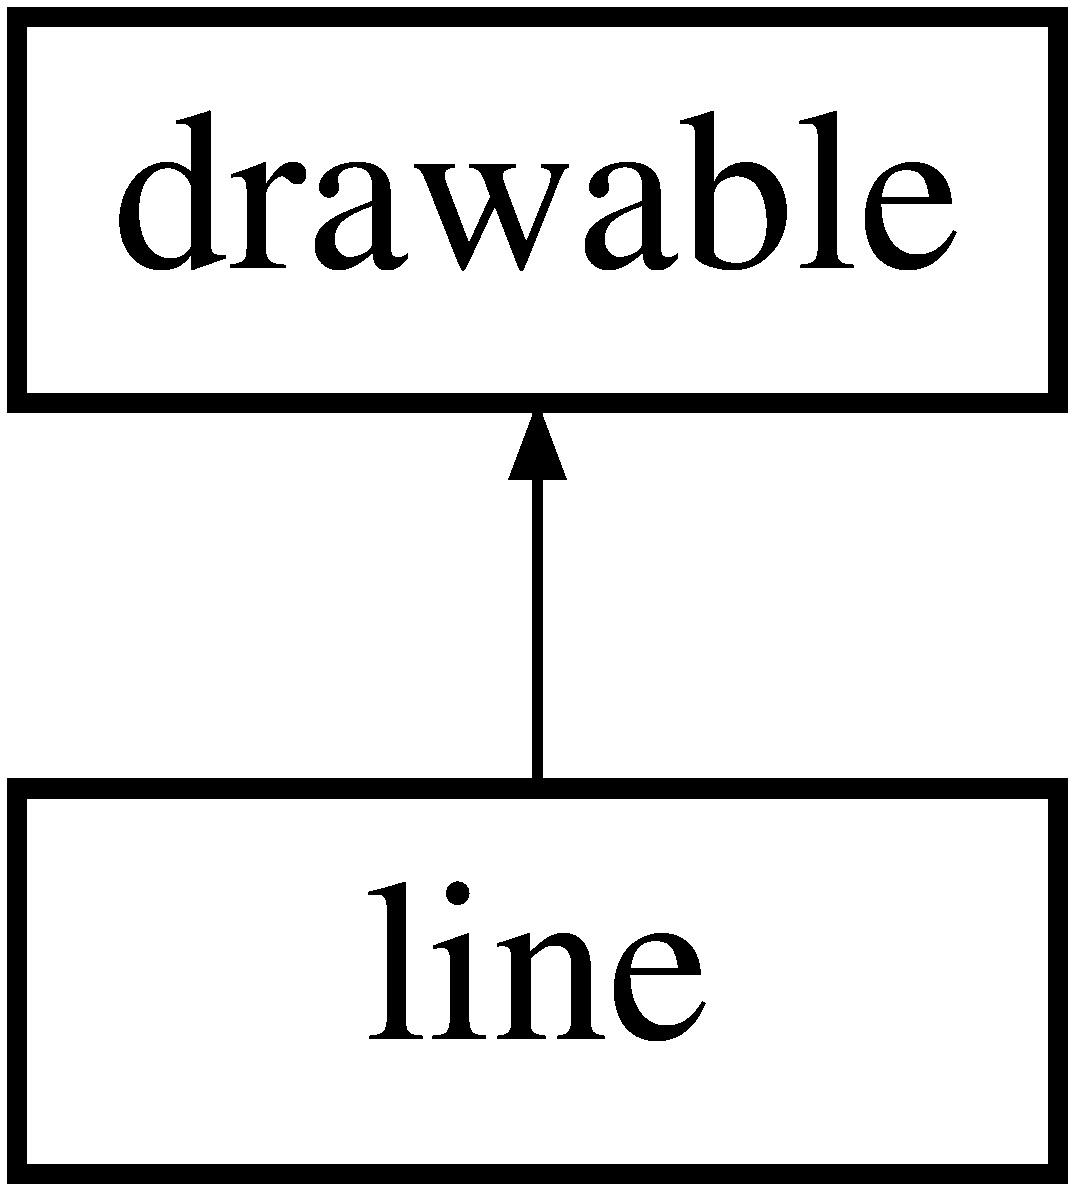
\includegraphics[height=2.000000cm]{classline}
\end{center}
\end{figure}
\subsection*{Public Member Functions}
\begin{DoxyCompactItemize}
\item 
\mbox{\Hypertarget{classline_a43ea2acfb458b795c9958508dadd9d18}\label{classline_a43ea2acfb458b795c9958508dadd9d18}} 
{\bfseries line} (\hyperlink{classwindow}{window} \&w, const \hyperlink{classvector}{vector} \&location, const \hyperlink{classvector}{vector} \&end)
\item 
\mbox{\Hypertarget{classline_af667c8ab35370df5d90e595cfb647c72}\label{classline_af667c8ab35370df5d90e595cfb647c72}} 
void {\bfseries draw} () override
\end{DoxyCompactItemize}
\subsection*{Additional Inherited Members}


The documentation for this class was generated from the following files\+:\begin{DoxyCompactItemize}
\item 
line.\+hpp\item 
line.\+cpp\end{DoxyCompactItemize}

\hypertarget{classstructure}{}\section{structure Class Reference}
\label{classstructure}\index{structure@{structure}}


structure  




{\ttfamily \#include $<$structure.\+hpp$>$}

\subsection*{Public Member Functions}
\begin{DoxyCompactItemize}
\item 
\hyperlink{classstructure_a0ed33e802c75a39ae0ea4f32591801d6}{structure} (\hyperlink{classwindow}{window} \&w, int row, int column)
\begin{DoxyCompactList}\small\item\em The constructor of a structure. \end{DoxyCompactList}\item 
void \hyperlink{classstructure_a0ea72a58f3ccac0a64a0f9b676c1776c}{print} ()
\begin{DoxyCompactList}\small\item\em a print function of a structure \end{DoxyCompactList}\end{DoxyCompactItemize}


\subsection{Detailed Description}
structure 

this library contains a c++ and a h++ file, it contains a constructor and a print function for a structure made out of rows and columns 

\subsection{Constructor \& Destructor Documentation}
\mbox{\Hypertarget{classstructure_a0ed33e802c75a39ae0ea4f32591801d6}\label{classstructure_a0ed33e802c75a39ae0ea4f32591801d6}} 
\index{structure@{structure}!structure@{structure}}
\index{structure@{structure}!structure@{structure}}
\subsubsection{\texorpdfstring{structure()}{structure()}}
{\footnotesize\ttfamily structure\+::structure (\begin{DoxyParamCaption}\item[{\hyperlink{classwindow}{window} \&}]{w,  }\item[{int}]{row,  }\item[{int}]{column }\end{DoxyParamCaption})\hspace{0.3cm}{\ttfamily [inline]}}



The constructor of a structure. 

This is a constructor that makes a strucure from two parameters it the rows and columns determine how many times the structure is printed 

\subsection{Member Function Documentation}
\mbox{\Hypertarget{classstructure_a0ea72a58f3ccac0a64a0f9b676c1776c}\label{classstructure_a0ea72a58f3ccac0a64a0f9b676c1776c}} 
\index{structure@{structure}!print@{print}}
\index{print@{print}!structure@{structure}}
\subsubsection{\texorpdfstring{print()}{print()}}
{\footnotesize\ttfamily void structure\+::print (\begin{DoxyParamCaption}{ }\end{DoxyParamCaption})}



a print function of a structure 

this function makes a structure of rectangles, lines and circles and prints this structure the column and row determine how many times it is printed 

The documentation for this class was generated from the following files\+:\begin{DoxyCompactItemize}
\item 
\hyperlink{structure_8hpp}{structure.\+hpp}\item 
structure.\+cpp\end{DoxyCompactItemize}

\hypertarget{classwindow}{}\section{window Class Reference}
\label{classwindow}\index{window@{window}}
\subsection*{Public Member Functions}
\begin{DoxyCompactItemize}
\item 
\mbox{\Hypertarget{classwindow_a26b54741901955b42941d3e08f09ba83}\label{classwindow_a26b54741901955b42941d3e08f09ba83}} 
{\bfseries window} (int x\+\_\+size, int y\+\_\+size, int scale)
\item 
\mbox{\Hypertarget{classwindow_a20541f9e1801404baf9a9184365e9b93}\label{classwindow_a20541f9e1801404baf9a9184365e9b93}} 
void {\bfseries draw} (int x, int y)
\item 
\mbox{\Hypertarget{classwindow_a6c050475db28a9b773cf2edbc56ece86}\label{classwindow_a6c050475db28a9b773cf2edbc56ece86}} 
void {\bfseries clear} ()
\end{DoxyCompactItemize}


The documentation for this class was generated from the following files\+:\begin{DoxyCompactItemize}
\item 
window.\+hpp\item 
window.\+cpp\end{DoxyCompactItemize}

\chapter{File Documentation}
\hypertarget{structure_8hpp}{}\section{structure.\+hpp File Reference}
\label{structure_8hpp}\index{structure.\+hpp@{structure.\+hpp}}
{\ttfamily \#include $<$iostream$>$}\newline
{\ttfamily \#include \char`\"{}window.\+hpp\char`\"{}}\newline
{\ttfamily \#include \char`\"{}filled\+\_\+rectangle.\+hpp\char`\"{}}\newline
{\ttfamily \#include \char`\"{}circle.\+hpp\char`\"{}}\newline
{\ttfamily \#include \char`\"{}line.\+hpp\char`\"{}}\newline
\subsection*{Classes}
\begin{DoxyCompactItemize}
\item 
class \hyperlink{classstructure}{structure}
\begin{DoxyCompactList}\small\item\em structure \end{DoxyCompactList}\end{DoxyCompactItemize}

%--- End generated contents ---

% Index
\backmatter
\newpage
\phantomsection
\clearemptydoublepage
\addcontentsline{toc}{chapter}{Index}
\printindex

\end{document}
